% Checkpoint 2: preparação e limpeza dos dados (frente B, base comum das duas frentes).
% Mesmo template do checkpoint 1: UFGTeX-Presentation (github.com/deuslirio/UFGTeX-Presentation).
% Tema e imagens copiados sem alteração de reports/slides/checkpoint1-ambiente/ (branch cnn/ambiente-gpu).
% Compilar nesta pasta: pdflatex checkpoint2-dados.tex (duas vezes, por causa da numeração),
% ou tectonic checkpoint2-dados.tex, ou subir a pasta no Overleaf.
% Figuras: python scripts/make_checkpoint2_figures.py (gera ../../figures/*.pdf).
\documentclass[aspectratio=169,t,xcolor=table]{beamer}
\usepackage[utf8]{inputenc}
\usepackage[brazil]{babel}
\usepackage{booktabs}
\usepackage{listings}

\usetheme{Ufg}
\usetikzlibrary{positioning}
% No repositório as figuras ficam em reports/figures/; no Overleaf, suba-as numa pasta figs/ ao lado deste .tex.
\graphicspath{{../../figures/}{figs/}}

\setPrimaryColor{UFGBlue}
\setLogos{lib/logos/INF-compact-white.png}{lib/logos/INF-compact-white.png}

% Cores das fases (as mesmas do diagrama de blocos do checkpoint 1)
\definecolor{PhaseOne}{RGB}{33, 33, 33}
\definecolor{PhaseNN}{RGB}{0, 114, 185}
\definecolor{PhaseClassic}{RGB}{214, 122, 0}
\definecolor{PhaseEval}{RGB}{91, 141, 8}

\newcommand{\code}[1]{\texttt{#1}}

\begin{document}

%==========================================================
% Capa (mesma estrutura do checkpoint 1)
\title{Preparação e Limpeza dos Dados}
\subtitle{Reconhecimento de Emoções em Imagens Faciais: a base comum das duas frentes}
\author{%
    \begin{tabular}{r@{\hspace{0.4em}}l@{\hspace{2.2em}}r@{\hspace{0.4em}}l}
        Antonio H. Q. V. Lopes & {\mdseries(202503993)} & Kauã L. Sandes    & {\mdseries(202504016)} \\
        Luccas J. R. Clemente  & {\mdseries(202504019)} & Yago L. Coqueiro & {\mdseries(202504028)} \\
    \end{tabular}}
\institute{INF0413 -- Processamento de Sinal e Imagem $\cdot$ Prof. Aldo Díaz\\
    Instituto de Informática $\cdot$ Universidade Federal de Goiás\\
    github.com/KauaSandes/seminario-reconhecimento-emocoes}
\date{Prévia do Seminário $\cdot$ Checkpoint 2 $\cdot$ Novembro de 2026}

\frame[noframenumbering]{\titlepage}

%==========================================================
\setLayout{vertical}
\begin{frame}{1. Onde estamos}

    \centering
    \begin{tikzpicture}[
            box/.style={rectangle, rounded corners=3pt, minimum width=3.0cm, minimum height=0.95cm,
                    align=center, font=\scriptsize, text=white, inner sep=2pt},
            phase/.style={font=\scriptsize\bfseries, align=right, anchor=east},
            arr/.style={->, >=stealth, draw=LightGray, thick},
            node distance=0.45cm]
        % Fase 1: em destaque (concluída nesta rodada)
        \node[box, fill=PhaseOne] (b1) {\textbf{Bases}\\FER-2013 e CK+};
        \node[box, fill=PhaseOne, right=of b1] (b2) {\textbf{Limpeza}\\duplicatas, rótulos, vazias};
        \node[box, fill=PhaseOne, right=of b2] (b3) {\textbf{Divisão}\\treino, validação, teste};
        \node[phase, text=PhaseOne] at ([xshift=-0.25cm]b1.west) {Fase 1\\Preparar\\os dados};
        \draw[arr, draw=PhaseOne] (b1) -- (b2);
        \draw[arr, draw=PhaseOne] (b2) -- (b3);
        % Fases seguintes: esmaecidas
        \begin{scope}[opacity=0.35, text opacity=0.6]
            \node[box, fill=PhaseNN, below=0.35cm of b1] (n1) {CNN do zero};
            \node[box, fill=PhaseNN, right=of n1] (n2) {Transfer learning};
            \node[box, fill=PhaseNN, right=of n2] (n3) {Vídeo: CNN + LSTM};
            \node[box, fill=PhaseClassic, below=0.2cm of n1] (c1) {Pré-processamento};
            \node[box, fill=PhaseClassic, right=of c1] (c2) {Descritores};
            \node[box, fill=PhaseClassic, right=of c2] (c3) {SVM e k-NN};
            \node[box, fill=PhaseEval, below=0.35cm of c1] (e1) {Métricas};
            \node[box, fill=PhaseEval, right=of e1] (e2) {Robustez};
            \node[box, fill=PhaseEval, right=of e2] (e3) {Interpretação};
            \node[phase, text=PhaseNN] at ([xshift=-0.25cm]n1.west) {Fase 2a};
            \node[phase, text=PhaseClassic] at ([xshift=-0.25cm]c1.west) {Fase 2b};
            \node[phase, text=PhaseEval] at ([xshift=-0.25cm]e1.west) {Fase 3};
        \end{scope}
    \end{tikzpicture}

    \raggedright
    \begin{block}{Esta rodada: a Fase 1, que as duas frentes compartilham}
        Mesmos dados, mesma limpeza, mesma divisão e mesmas métricas para redes e clássicos.
    \end{block}

\end{frame}

%==========================================================
\begin{frame}{2. Obtenção dos dados}

    \begin{table}[]
        \centering
        \footnotesize
        \renewcommand{\arraystretch}{1.3}
        \setlength{\tabcolsep}{7pt}
        {\rowcolors{2}{}{LightGray!10}
            \begin{tabular}{>{\raggedright\arraybackslash}p{1.6cm}>{\raggedright\arraybackslash}p{4.6cm}>{\raggedright\arraybackslash}p{4.4cm}}
                \toprule
                           & \textbf{FER-2013}                            & \textbf{CK+}                                \\
                \midrule
                Fonte      & Competição oficial do Kaggle                  & Pedido aos autores (Lucey et al., 2010)     \\
                Conteúdo   & 35.887 rostos 48$\times$48, 7 classes         & 593 sequências, 327 rotuladas               \\
                Divisão    & oficial: 28.709 / 3.589 / 3.589               & 10 partes, agrupadas por pessoa             \\
                Situação   & \textcolor{DarkGreen}{\textbf{baixada e validada}} (SHA-256) & \textcolor{DarkOrange}{\textbf{aguardando acesso}}; código pronto e testado \\
                \bottomrule
            \end{tabular}
        }
    \end{table}

    \begin{alertblock}{Por que não usar as cópias em pastas de imagens}
        Versões como a \code{msambare/fer2013} perderam a separação PublicTest/PrivateTest:\\
        a validação e o teste oficiais deixariam de existir.
    \end{alertblock}\par
    \vspace{\fill}

\end{frame}

%==========================================================
\begin{frame}{3. A base comum: \code{src/common}}

    \begin{table}[]
        \centering
        \footnotesize
        \renewcommand{\arraystretch}{1.3}
        \setlength{\tabcolsep}{7pt}
        {\rowcolors{2}{}{LightGray!10}
            \begin{tabular}{>{\raggedright\arraybackslash}p{1.8cm}>{\raggedright\arraybackslash}p{4.5cm}>{\raggedright\arraybackslash}p{4.3cm}}
                \toprule
                \textbf{Módulo}    & \textbf{O que oferece}                          & \textbf{O que garante}               \\
                \midrule
                \code{data.py}     & \code{load\_fer2013}, \code{load\_ckplus}       & os mesmos dados para todos            \\
                \code{clean.py}    & limpeza e \code{class\_weights}                 & a mesma limpeza para todos            \\
                \code{degrade.py}  & ruído, desfoque e resolução                     & as mesmas degradações                 \\
                \code{metrics.py}  & \code{evaluate}, \code{save\_results}           & um só formato de resultado            \\
                \bottomrule
            \end{tabular}
        }
    \end{table}

    \begin{block}{Dois comandos preparam tudo}
        \code{python scripts/download\_data.py} \hfill baixa, extrai e valida\\
        \code{python -m src.common.prepare\_data} \hfill limpa, divide e relata
    \end{block}\par
    \vspace{\fill}

\end{frame}

%==========================================================
\begin{frame}{4. Limpeza: o que procuramos}

    \begin{table}[]
        \centering
        \footnotesize
        \renewcommand{\arraystretch}{1.25}
        \setlength{\tabcolsep}{7pt}
        {\rowcolors{2}{}{LightGray!10}
            \begin{tabular}{>{\raggedright\arraybackslash}p{4.9cm}>{\raggedright\arraybackslash}p{2.6cm}>{\raggedright\arraybackslash}p{2.9cm}}
                \toprule
                \textbf{Problema}                          & \textbf{Treino}       & \textbf{Validação e teste} \\
                \midrule
                Duplicata exata (mesmos pixels)            & fica uma cópia        & só sinaliza                \\
                Cópia de imagem da validação/teste         & sai (vazamento)       & intactas                   \\
                Cópias com rótulos diferentes              & saem                  & só sinaliza                \\
                Imagem vazia (desvio padrão $<$ 5)         & sai                   & só sinaliza                \\
                Sem rosto detectado (Viola-Jones)          & só sinaliza           & só sinaliza                \\
                \bottomrule
            \end{tabular}
        }
    \end{table}

    \begin{block}{Nada é apagado}
        O arquivo versionado \code{splits/fer2013\_clean.csv} diz o que entra. Validação e teste\\
        ficam intactos, comparáveis com a literatura.
    \end{block}\par
    \vspace{\fill}

\end{frame}

%==========================================================
\setLayout{blank}
\setBGColor{UFGBlue}
\begin{frame}{5. Limpeza: resultado}

    \vspace{1.0cm}
    \begin{columns}[c]
        \column{0.3\textwidth}  \stat{26.911}{imagens de treino\\(eram 28.709)}
        \column{0.03\textwidth} \statsep
        \column{0.3\textwidth}  \stat{703}{cópias de imagens da\\validação e do teste}
        \column{0.03\textwidth} \statsep
        \column{0.3\textwidth}  \stat{0}{alterações na\\validação e no teste}
    \end{columns}

    \vspace{1.0cm}
    {\footnotesize 1.798 imagens saíram do treino (6,3\%). Sem a limpeza, 703 imagens de avaliação já teriam\\
    sido vistas no treino, e a acurácia medida ficaria otimista.}

\end{frame}

%==========================================================
\setLayout{vertical}
\begin{frame}{6. O que saiu do treino}

    \centering
    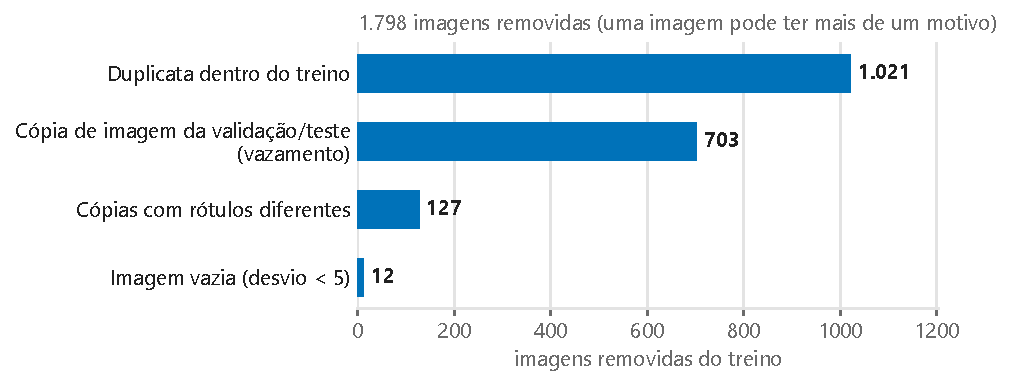
\includegraphics[height=4.6cm]{fer2013_cleaning_removals_by_reason.pdf}

    \raggedright
    \begin{block}{}
        As duplicatas se concentram em \textbf{surpresa}: 711 das 1.798 imagens removidas.
    \end{block}

\end{frame}

%==========================================================
\begin{frame}{7. Imagens vazias e o limiar}

    \centering
    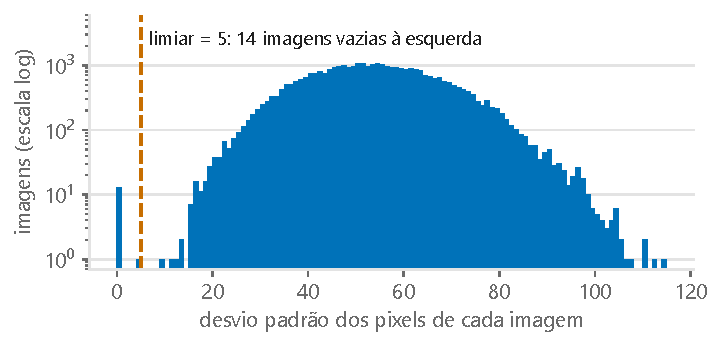
\includegraphics[height=4.3cm]{fer2013_std_histogram.pdf}

    \raggedright
    \begin{block}{O desvio padrão dos pixels mede o contraste: 0 é uma imagem lisa}
        Há um vão natural entre 4,1 e 9,1. O limiar 5 pega as 14 imagens vazias (12 no treino)\\
        e preserva todos os rostos. Conferido visualmente antes de ser fixado.
    \end{block}

\end{frame}

%==========================================================
\begin{frame}{8. Distribuição de classes}

    \centering
    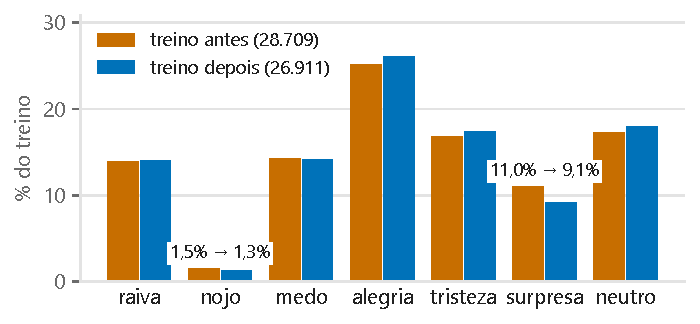
\includegraphics[height=4.3cm]{fer2013_class_distribution.pdf}

    \raggedright
    \begin{block}{O desbalanceamento continua: nojo tem 1,3\% do treino}
        \code{class\_weights(y)} (inverso da frequência, igual ao \emph{balanced} do scikit-learn)\\
        dá peso 10,98 ao nojo e 0,55 à alegria, nas duas frentes.
    \end{block}

\end{frame}

%==========================================================
\begin{frame}{9. Robustez: degradações prontas}

    \begin{columns}[T]
        \column{0.47\textwidth}
        \centering
        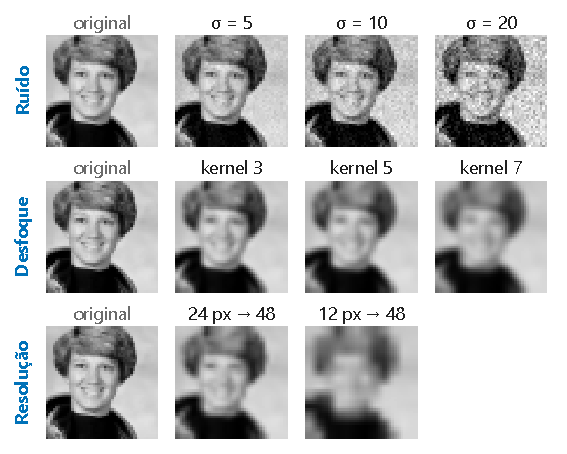
\includegraphics[height=5.6cm]{degradations_example_face.pdf}\\[-0.1em]
        {\tiny Rosto de exemplo: imagem \emph{astronaut} do scikit-image (domínio público).}

        \column{0.46\textwidth}
        \vspace{0.3cm}
        \begin{itemize}
            \item Aplicadas \textbf{só no teste}
            \item Mesmos níveis e mesma semente nas duas frentes
            \item Ruído gaussiano: tema do \textbf{le03}
            \item Resolução: média por área (antialias) e volta a 48 px; amostragem e Nyquist do \textbf{le04}
        \end{itemize}

        \vspace{0.4cm}
        \begin{block}{}
            Saída: curvas de acurácia por nível, redes contra clássicos.
        \end{block}
    \end{columns}

\end{frame}

%==========================================================
\begin{frame}{10. Qualidade e reprodutibilidade}

    \begin{table}[]
        \centering
        \footnotesize
        \renewcommand{\arraystretch}{1.3}
        \setlength{\tabcolsep}{8pt}
        {\rowcolors{2}{}{LightGray!10}
            \begin{tabular}{>{\raggedright\arraybackslash}p{3.4cm}>{\raggedright\arraybackslash}p{7.2cm}}
                \toprule
                \textbf{Garantia}        & \textbf{Como}                                                        \\
                \midrule
                Código testado           & 87 testes automáticos (pytest)                                      \\
                Mesmo arquivo em toda máquina & SHA-256 do \code{fer2013.csv} conferido pelo script              \\
                Resultados comparáveis   & seed 42 e um único JSON de métricas                                 \\
                Sem dados no GitHub      & cada um baixa da fonte oficial                                      \\
                \bottomrule
            \end{tabular}
        }
    \end{table}

    \begin{block}{Primeira linha de base: classe majoritária}
        Prever sempre ``alegria'' acerta \textbf{24,9\%} da validação (F1 macro 0,06).\\
        É o piso para todos os métodos.
    \end{block}\par
    \vspace{\fill}

\end{frame}

%==========================================================
\begin{frame}{11. Próximos passos}

    \begin{itemize}
        \item \textbf{Frente B:} pré-processamento (Viola-Jones, equalização, gaussiano) e os descritores Gabor, HOG, LBP e DCT
        \item \textbf{Frente A:} ligar o pipeline à base comum e treinar a CNN do zero e a ResNet-18
        \item \textbf{CK+:} aguardando a resposta dos autores; o código já está pronto e testado
        \item Revisão cruzada da base comum e merge na \code{main}
    \end{itemize}

    \vspace{0.6em}
    \begin{block}{Situação}
        A base comum está pronta: as duas frentes já podem treinar sobre os mesmos dados.
    \end{block}

\end{frame}

%==========================================================
\setLayout{blank}
\setBGColor{UFGBlue}
\setbeamertemplate{footline}[ftln]
\begin{frame}[noframenumbering]

    \centering
    \vspace{2cm}

    \textbf{\Huge Obrigado}

    \ \\

    \textbf{Dúvidas e sugestões}

    \vspace{1cm}
    \begin{figure}
        \centering
        
\includegraphics[height=3cm]{lib/logos/INF-full-white.png}
    \end{figure}

\end{frame}

\end{document}
